\documentclass{lehramt-informatik-haupt}
\liLadePakete{mathe}
\usepackage{tikz}
\usetikzlibrary{calc,trees,positioning,arrows,fit,shapes,calc}

\begin{document}

%%%%%%%%%%%%%%%%%%%%%%%%%%%%%%%%%%%%%%%%%%%%%%%%%%%%%%%%%%%%%%%%%%%%%%%%
% Theorie-Teil
%%%%%%%%%%%%%%%%%%%%%%%%%%%%%%%%%%%%%%%%%%%%%%%%%%%%%%%%%%%%%%%%%%%%%%%%

\chapter{Berechbarkeitstheorie}

\begin{liQuellen}
\item \cite[Seite 253-340]{hoffmann}
\end{liQuellen}

\subsection{Berechenbarkeitsmodelle}

%%
%
%%

% Info_2021-05-07-2021-05-07_09.32.08.mp4 1h

\subsubsection{Loop-berechenbar}

\begin{liQuellen}
\item \cite[Seite 7-11]{theo:fs:4}
\item \cite[Seite 254-260]{hoffmann}
\item \cite{wiki:loop}
\end{liQuellen}

\paragraph{LOOP-Sprache (einfache Programme)}

\begin{itemize}
\item endlicher Aufbau
\item Variablen aus den natürlichen Zahlen
\end{itemize}

\begin{description}
\item[Programmelemente:] \strut

\begin{description}
\item[Konstante:]
$0$ (andere Kostanten müssen aus den anderen Element )

\item[Variablen:]
$x_0, x_1, x_2, \dots, x_n$

\item[Operator:]

$succ$ (Successor), $pred$ (Sredecessor), $:=$ (Wertzuweisen), $;$ (Anweisungtrenner)

\item[Schleife:]

$loop \dots do \dots end$ (nach dem loop Schlüsselwort steht genau eine
Variable, die dekrementiert wird. Ist 0 erreicht, stop die Schleife)
\end{description}

\item[Speichervektor v:] \strut

\begin{itemize}
\item endlich, aber beliebig lang
\item Speicherung der Variablen des Programms
\item $(x_0, x_1, x_2, \dots, x_n)$
\item Erste Stelle des Vektors ist für das Speichern des Ergebnisses vorgesehen.
\end{itemize}

\item[Übergangsfunktion $\delta(v, P)$:] \strut

\begin{description}
\item[Eingabe:] Speichervektor $v$ und Programm $P$
\item[Ausgabe:] Speichervektor $v'$
\end{description}

nach Programmausführung von $P$

\item[Makro] \strut

Es gibt die Möglichkeit sogenannte Makros zu definieren.
\end{description}

%%
%
%%

% Info_2021-05-07-2021-05-07_09.32.08.mp4 2h

\subsubsection{While-Programme}

\begin{liQuellen}
\item \cite[Seite 7-12]{theo:fs:4}
\item \cite[Seite 260-264]{hoffmann}
\item \cite{wiki:while}
\end{liQuellen}

\begin{itemize}
\item endlicher Aufbau
\item Variablen aus den natürlichen Zahlen
\end{itemize}

\begin{description}
\item[Programmelemente:] \strut

\begin{description}
\item[Konstante:]
$0$ (andere Kostanten müssen aus den anderen Element )

\item[Variablen:]
$x_0, x_1, x_2, \dots, x_n$

\item[Operator:]

$succ$ (Successor), $pred$ (Predecessor), $:=$ (Wertzuweisen), $;$ (Anweisungtrenner)

\item[Schleife:]

 $loop \dots do \dots end$(nach dem $loop$ Schlüsselwort steht genau eine
Variable, die dekrementiert wird. Ist 0 erreicht, stop die Schleife)

\item[Schleife:]

$while \dots do \dots end$
(nach dem $while$ Schlüsselwort steht eine Bedingung. $while$-Schleife
kann nicht terminieren.)
\end{description}

\item[Speichervektor v:] \strut

\begin{itemize}
\item endlich, aber beliebig lang
\item Speicherung der Variablen des Programms
\item $(x_0, x_1, x_2, \dots, x_n)$
 \end{itemize}

\item[Übergangsfunktion $\delta(v, P)$:] \strut

\begin{description}
\item[Eingabe:] Speichervektor $v$ und Programm $P$
\item[Ausgabe:] Speichervektor $v'$
\end{description}

nach Programmausführung von $P$
\begin{equation*}
\delta(v, \text{while }x_i\text{ do }P)
\begin{cases}
\bot & \text{falls }T_i = \emptyset\\
\delta(v, P^{\text{min}T_i}) & \text{falls }T_i \neq \emptyset\\
\end{cases}
\end{equation*}
\end{description}

Mit $f : \mathbb{N}^n \rightarrow \mathbb{N}$ sei eine partielle
Funktion über den natürlichen Zahlen gegeben. $f$ heißt
While-berechenbar, falls ein While-Programm $P$ mit den folgenden
Eigenschaften existiert:

Satz von Kleene:

Jede WHILE-berechenbare Funktion lässt sich als WHILE-Programm mit nur
einer WHILE-Schleife realisieren.\footcite[Seite 13]{theo:fs:4}

\subsection{Weitere Berechnungsmodelle}

\begin{itemize}
\item GOTO
\item primitive und μ-Rekursion

\item Turing-Maschinen
\begin{itemize}
\item Einband-TM
\item Mehrband-TM
\item Universelle-TM

\end{itemize}
\item Registermaschinen
\item lambda-Kalkül\footcite[Seite 17]{theo:fs:4}
\end{itemize}

\section{Universelle Turingmaschine}

% Info_2021-05-07-2021-05-07_09.32.08.mp4 2h47min

Eine Turing-Maschine $U$ heißt universell, wenn sie eine andere
Turing-Maschine $T$ simulieren (ausführen) kann.\footcite[Seite
23]{theo:fs:4}

\begin{equation*}
\delta((0,x_1,x_2,\dots,x_n,0,\dots), P) =
\begin{cases}
\bot &
\text{falls } f(x_1,x_2,\dots,x_n) = \bot\\

(f(x_1,x_2,\dots,x_n), \dots) &
\text{falls }f(x_1,x_2,\dots,x_n) \neq \bot\\
\end{cases}
\end{equation*}\footcite[Seite 261]{hoffmann}

\subsection{Gödelisierung:}

Für jeden Eintrag der Übergangstabelle wird eine Binärzahl erzeugt.
Startzustand, Eingabesymbol, Folgesymbol, Ausgabesymbol und Richtung
werden als Einserketten unär kodiert mit Null als Trennzeichen Nach dem
gleichen Schema werden die erstellten Bitsequenzen zu einer großen
Binärzahl verschmolzen. Die erzeugte Zahl heißt die \memph{Gödelnummer}
der TM $T$. Die Kodierung wird als \memph{Gödelisierung} bezeichnet.
\footcite[Seite 23]{theo:fs:4}

\subsection{Church‘sche These}
\footcite{wiki:church-these}

Die Klasse der turing-berechenbaren Funktionen stimmt mit der
Klasse der intuitiv berechenbaren Funktionen überein.

Der Begriff der intuitiv berechenbaren Funktion bedarf an dieser Stelle
besonderer Aufmerksamkeit. Er bezeichnet eine Funktion, die von einem
Menschen – in welcher Form auch immer – ausgerechnet werden kann. Damit
besagt die Church’sche These nichts anderes, als dass je- de Funktion,
die überhaupt in irgendeiner Weise berechenbar ist, auch durch eine
Turing-Maschine berechnet werden kann. Die Church’sche These ist kein
Satz im mathematisch präzisen Sinne, da der Begriff der intuitiv
berechenbaren Funktion keine formale Definition besitzt. Gäbe es
diese, so hätten wir uns – bewusst oder unbewusst – bereits auf ein
konkretes Berechnungsmodell festgelegt und die eigentliche Bedeutung
dieses Begriffs ad absurdum geführt. Folgerichtig wird es niemals
möglich sein, die Church’sche These zu beweisen. Wir können lediglich
Indizien für ihre Gültigkeit sammeln und genau dies ist Forschern in der
Vergangenheit vielfach gelungen.
\footcite[Seite 308]{hoffmann}

Intuitiv-berechenbar:
Funktionen, die von einem Menschen berechnet werden können.

Church‘sche These kann nicht bewiesen werden!
\footcite[Seite 27]{theo:fs:4}

\begin{liExkurs}[Funktion]
In der Mathematik ist eine Funktion (lateinisch functio) oder Abbildung
eine Beziehung (Relation) zwischen zwei Mengen, die jedem Element der
einen Menge (Funktionsargument, unabhängige Variable, $x$-Wert) genau
ein Element der anderen Menge (Funktionswert, abhängige Variable,
$y$-Wert) zuordnet.
\liFussnoteUrl{https://de.wikipedia.org/wiki/Funktion_(Mathematik)}

Eine (totale) Funktion ist eine Relation $R \subseteq M \times N$ über dem
Definitionsbereich $M$ und dem Wertebereich $N$, welche folgende
Eigenschaften hat:

\begin{enumerate}
\item Jedes Element aus dem Definitionsbereich $M$ ist mit höchstens
einem Element aus dem Wertebereich $N$ verbunden. (\emph{rechtseindeutig})

\item Jedes Element von $M$ ist mit einem Element aus $N$ verbunden.
(\emph{linkstotal})
\end{enumerate}
\liFussnoteUrl{https://files.ifi.uzh.ch/cl/siclemat/lehre/ws0607/ecl1/script/html/scriptse48.html}
\end{liExkurs}

\begin{liExkurs}[Totale Funktion]
Eine rechtseindeutige bzw. funktionale Relation nennt man auch partielle
Funktion. Wenn diese auch linkstotal – also eine Funktion – ist, dann
sagt man zur Verdeutlichung auch totale Funktion.
\liFussnoteUrl{https://de.wikipedia.org/wiki/Relation_(Mathematik)}
\end{liExkurs}

\begin{liExkurs}[Partielle Funktion]
Der Begriff der partiellen Funktion ist eine Verallgemeinerung des
Begriffs der Funktion. Unter einer Funktion von $X$ nach $Y$ versteht
man eine linkstotale, rechtseindeutige Relation, also eine Relation, in
der jedem Element von $X$ genau ein Element von $Y$ zugeordnet ist. Jede
Funktion von $X$ nach $Y$ ist also insbesondere eine partielle Funktion
von $X$ nach $Y$, nämlich eine (links-)totale partielle Funktion, aber
nicht umgekehrt. Insofern kann der Begriff der partiellen Funktion
irreführend sein. Um auszudrücken, dass eine partielle Funktion sogar
eine Funktion im eigentlichen Sinn ist, sagt man gelegentlich, es handle
sich um eine totale Funktion. Der Unterschied zwischen partiellen
Funktionen und (totalen) Funktionen ist: Für partielle Funktionen

\begin{displaymath}
f\colon \;X \rightharpoonup Y
\end{displaymath}

\noindent
gilt

\begin{displaymath}
\operatorname {Def} (f) \subseteq X ,
\end{displaymath}

\noindent
für (totale) Funktionen

\begin{displaymath}
f \colon \; X \to Y
\end{displaymath}

 gilt

\begin{displaymath}
\operatorname {Def} (f)=X .
\end{displaymath}

\liFussnoteUrl{https://de.wikipedia.org/wiki/Partielle_Funktion}
\end{liExkurs}

 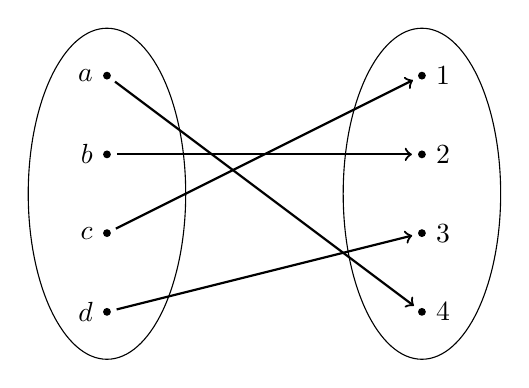
\begin{tikzpicture}[ele/.style={fill=black,circle,minimum width=.8pt,inner sep=1pt},every fit/.style={ellipse,draw,inner sep=-2pt}]
  \node[ele,label=left:$a$] (a1) at (0,4) {};
  \node[ele,label=left:$b$] (a2) at (0,3) {};
  \node[ele,label=left:$c$] (a3) at (0,2) {};
  \node[ele,label=left:$d$] (a4) at (0,1) {};

  \node[ele,,label=right:$1$] (b1) at (4,4) {};
  \node[ele,,label=right:$2$] (b2) at (4,3) {};
  \node[ele,,label=right:$3$] (b3) at (4,2) {};
  \node[ele,,label=right:$4$] (b4) at (4,1) {};

  \node[draw,fit= (a1) (a2) (a3) (a4),minimum width=2cm] {} ;
  \node[draw,fit= (b1) (b2) (b3) (b4),minimum width=2cm] {} ;
  \draw[->,thick,shorten <=2pt,shorten >=2pt] (a1) -- (b4);
  \draw[->,thick,shorten <=2pt,shorten >=2] (a2) -- (b2);
  \draw[->,thick,shorten <=2pt,shorten >=2] (a3) -- (b1);
  \draw[->,thick,shorten <=2pt,shorten >=2] (a4) -- (b3);
 \end{tikzpicture}

\literatur

\end{document}
